\documentclass[11pt]{article}

\usepackage{graphicx}
\usepackage{wrapfig}
\usepackage{url}
\usepackage{wrapfig}
\usepackage{color}
\usepackage{marvosym}
\usepackage{enumerate}
\usepackage{subfigure}
\usepackage{tikz}
\usepackage{amsmath}
\usepackage{amssymb}
\usepackage{hyperref} 
\usepackage{filecontents}
\usepackage{cite}
\usepackage{lastpage}
\usepackage{fancyhdr}
\usepackage{filecontents}


\oddsidemargin 0mm
\evensidemargin 5mm
\topmargin -20mm
\textheight 240mm
\textwidth 160mm
\setlength{\footskip}{20pt}
\newcommand{\captionfonts}{\small}
\newcommand{\vw}{{\bf w}}
\newcommand{\vx}{{\bf x}}
\newcommand{\vy}{{\bf y}}
\newcommand{\vxi}{{\bf x}_i}
\newcommand{\yi}{y_i}
\newcommand{\vxj}{{\bf x}_j}
\newcommand{\vxn}{{\bf x}_n}
\newcommand{\yj}{y_j}
\newcommand{\ai}{\alpha_i}
\newcommand{\aj}{\alpha_j}
\newcommand{\X}{{\bf X}}
\newcommand{\Y}{{\bf Y}}
\newcommand{\vz}{{\bf z}}
\newcommand{\msigma}{{\bf \Sigma}}
\newcommand{\vmu}{{\bf \mu}}
\newcommand{\vmuk}{{\bf \mu}_k}
\newcommand{\msigmak}{{\bf \Sigma}_k}
\newcommand{\vmuj}{{\bf \mu}_j}
\newcommand{\msigmaj}{{\bf \Sigma}_j}
\newcommand{\pij}{\pi_j}
\newcommand{\pik}{\pi_k}
\newcommand{\D}{\mathcal{D}}
\newcommand{\el}{\mathcal{L}}
\newcommand{\N}{\mathcal{N}}
\newcommand{\vxij}{{\bf x}_{ij}}
\newcommand{\vt}{{\bf t}}
\newcommand{\yh}{\hat{y}}
\newcommand{\code}[1]{{\footnotesize \tt #1}}
\newcommand{\alphai}{\alpha_i}

\newcommand\independent{\protect\mathpalette{\protect\independenT}{\perp}}
\def\independenT#1#2{\mathrel{\setbox0\hbox{$#1#2$}%
\copy0\kern-\wd0\mkern4mu\box0}}

\renewcommand{\figurename}{\tiny{Fig.}}
\renewcommand{\topfraction}{0.85}
\renewcommand{\textfraction}{0.1}

\begin{filecontents}{bibliography.bib}
@article{quake,
  title={Quake: quality-aware detection and correction of sequencing errors},
  author={David R Kelley, Michael C Schatz, Steven L Salzberg},
  journal={Genome Biology},
  volume={11},
  number={11},
  pages={13},
  year={2010}
}

@article{musket,
  title={Musket: a multistage k-mer spectrum based error corrector for Illumina sequence data},
  author={Yongchao Liu, Jan Schröder and Bertil Schmidt},
  journal={BioInformatics},
  year={2012},
  publisher={Oxford University Press}
}
@article{parallel,
  title={A parallel algorithm for error correction in high-throughput short-read data on CUDA-enabled graphics hardware},
  author={Shi H, Schmidt B, Liu W, Müller-Wittig W.},
  journal={Journal of Computational Biology},
  volume={17},
  number={4},
  year={2010},
  publisher={Mary Ann Liebert, Inc}
}
@article{bloom,
  title={Space/time trade-offs in hash coding with allowable errors},
  author={Burton H. Bloom},
  journal={Communications of the ACM},
  volume={13},
  number={7},
  pages={422--426},
  year={1970},
  publisher={ACM, New York}
}

@article{chikhi,
  title={Informed and Automated k-Mer Size Selection for Genome Assembly},
  author={Rayan Chikhi and Paul Medvedev},
  journal={BioInformatics},
  pages={1--7},
  year={2013}
}

@article{reptile,
  title={Reptile: representative tiling for short read error correction},
  author={Xiao Yang, Karin S. Dorman and Srinivas Aluru},
  journal={BioInformatics},
  volume={26},
  number={20},
  pages={2526--2533},
  year={2010}
}

@article{McGregor,
  title={Homomorphic Fingerprints under Misalignments: Sketching Edit and Shift Distances},
  author={Alexander Andoni, Assaf Goldberger, Andrew McGregor, Ely Porat},
  journal={STOC'13},
  year={2013},
  publisher={ACM}
}

@article{debruijn,
  title={A new algorithm for DNA sequence assembly.},
  author={Idury RM, Waterman MS.},
  journal={PubMed Central},
  volume={2},
  number={2},
  pages={291--306},
  year={1995},
  publisher={ACM}
}

@article{storm,
  title={Storm, Distributed and fault-tolerant realtime computation.},
  author={Nathan Marz},
  journal={https://github.com/nathanmarz/storm/wiki/Tutorial},
  year={2012}
}

\end{filecontents}

\begin{document}
\pagestyle{plain} 
\title{Quality-Aware, Parallel, Multistage Detection and Correction of Sequencing Errors using Storm}
\large
\date{}
\author{Lakshmisha Bhat (lbhat1@jhu.edu) \\Department of Computer Science, Johns Hopkins University \\[2\baselineskip]\\ }
\maketitle
\vspace{-.5in}
\cfoot{\thepage}
\rfoot{}
\rhead{}
\lhead{\tiny Quality-Aware, Parallel, Multistage Detection and Correction of Sequencing Errors using Storm}


\begin{abstract}
The sequence data produced by next-generation sequencing technologies are error-prone and has motivated the development of a number of short-read error correctors in recent years. The majority of methods focus on the correction of substitution errors, which are the dominant error source in data produced by Illumina sequencing technology. Our efforts are also aligned towards the same goal. We design a streaming pipeline that takes a stream of sequence reads, builds a distributed abundance histogram assisted by a distributed sketch and use this information to detect which read nucleotides are likely to be sequencing errors, all within the Storm ecosystem. Then, using a maximum likelihood approach, we correct errors by incorporating quality values to achieve the highest accuracy on realistically simulated reads.\\
\end{abstract}

\section{Introduction}
We saw earlier in the course that Sanger reads, typically 700 -- 1000 bp in length, are long enough for overlaps to be reliable indicators of genomic co-location, which are used in the overlap-layout-consensus approach for genome assembly. However, the de novo inference of a genome without the aid of a reference genome, is a hard problem to solve. The overlap-layout-consensus approach does poorly with the much shorter reads of second-generation sequencing platforms; for e.g. DNA sequence reads from Illumina sequencers, one of the most successful of the second-generation technologies, range from 35 to 125 bp in length. In this context, de Bruijn graph \cite{debruijn} based formulations that reconstruct the genome as a path in a graph perform better due to their more global focus and ability to naturally accommodate paired read information. As a result, it has become de facto model for building short-read genome assemblers. \\

In this setting it is worth talking about the correctness of these second-generation sequencers. It is well known that the sequence fidelity of these sequencers are high - they have a substitution error rate of 0.5--2.5 (empirically shown in \cite{quake}). Errors are attributed to templates getting “out of sync,” by missing an incorporation or by incorporating 2 or more nucleotides at once. These errors increase in the later sequencing cycles as proportionally more templates fall out of sync and hence their frequency at the 3' ends of reads is higher. This, as we shall see, becomes an important property to be considered for maximum likelihood estimation during error correction.\\

Error correction has long been recognized as a critical and difficult part of the so called graph-based assemblers (de Bruijn graph). It also has significant impact on alignment and in other next-generation sequencing applications such as re-sequencing. Sequencing errors complicate analysis, which normally requires that reads be aligned to each other during assemble or to a reference genome for single-nucleotide polymorphism (SNP) detection. Mistakes during the overlap computation in genome assembly may leave gaps in the assembly, while false overlaps may create ambiguous paths \cite{quake}. In genome re-sequencing projects, reads are aligned to a reference genome, usually allowing for a fixed number of mismatches due to either SNPs or sequencing errors. In most cases, the reference genome and the genome being newly sequenced will differ, sometimes substantially. Variable regions are more difficult to align because mismatches from both polymorphisms and sequencing errors occur, but if errors can be eliminated, more reads will align and the sensitivity for variant detection will improve.

Fortunately, the low cost of second-generation sequencing makes it possible to obtain highly redundant coverage of a genome, which can be used to correct sequencing errors in the reads before assembly or alignment. But, this significantly increases the size of the dataset. In order to deal with the computational challenges of working with such large data sets, a number of methods have been proposed for storing k-mers efficiently. Most de Bruijn graph assemblers store k-mers using 2 bits to encode each nucleotide, so that each k-mer takes $k/4$ bytes. The k-mers are then stored in a hash table, usually with some associated information such as coverage and neighborhood information in the de Bruijn graph. A complementary strategy for reducing memory usage is based on the observation that in current data sets, a large fraction of the observed k-mers may arise from sequencing errors. Most of these occur uniquely in the data, and hence they greatly increase the memory requirements of de novo assembly without adding much information. For this reason, it is frequently helpful to either discard unique k-mers prior to building the graph, or to attempt to correct them if they are similar to other, much more 'abundant', k-mers. A number of related methods have been proposed to perform this error correction step, all guided by the goal of finding the minimum number of single base edits (edit distance) to the read that make all k-mers trusted.



\section{Background}

\subsection{Bloom-Filter}
A Bloom filter \cite{bloom}, in simple terms, is a data structure designed to tell us, rapidly and memory-efficiently, whether an element is present in a set. The price paid for this efficiency is that a Bloom filter is probabilistic in nature: it tells us that the element is either definitely not in the set or 'may be' in the set.

\begin{figure}[ht!]
\centering
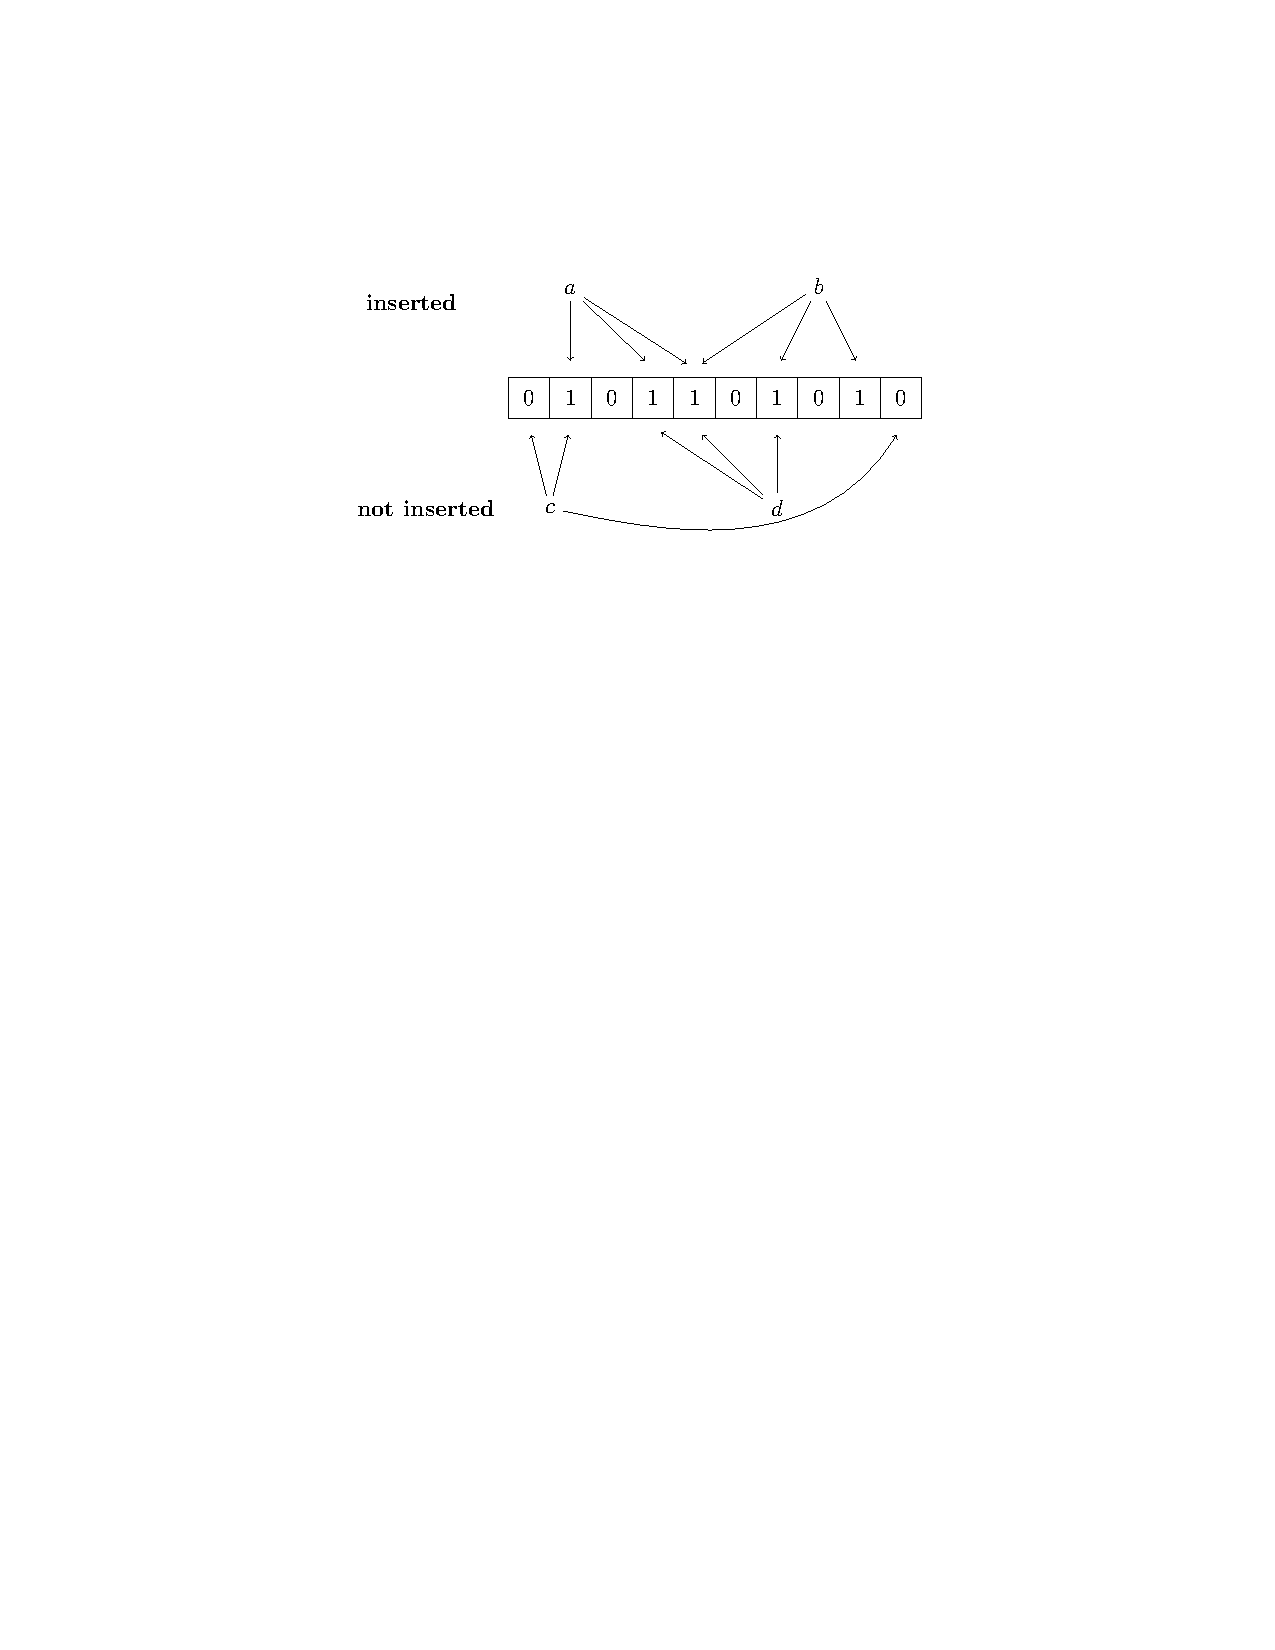
\includegraphics[width=90mm]{bloom.pdf}
\caption{\tiny{An example of a Bloom filter with three hash functions. The k-mers a and b have been inserted, but c and d have not. The Bloom filter indicates correctly that k-mer c has not been inserted since not all of its bits are set to 1. k-mer d has not been inserted, but since its bits were set to 1 by the insertion of a and b, the Bloom filter falsely reports that d has been seen already.}}
\label{overflow}
\end{figure}

More precisely, a Bloom filter is a method for representing a set $A = \{a_1, a_2, \ldots, a_n\}$ of n elements to support membership queries. The main idea is to allocate a vector 'v' of m bits, initially all set to 0, and then choose k independent hash functions, $h_1, h_2, \ldots, h_k$, each with range $\{1,\ldots,m\}$. For each element $a \in A$, the bits at positions h1(a), h2(a), ..., hk(a) in v are set to 1. Given a query for 'b' we check the bits at positions h1(b), h2(b), ..., hk(b). If any of them is 0, then certainly b is not in the set A. Otherwise we conjecture that b is in the set although there is a certain probability that we are wrong. This is called a 'false positive'. The parameters k and m should be chosen such that the probability of a false positive is acceptable. Perhaps the most critically acclaimed  feature of Bloom filters is that there is a clear trade-off between m and the probability of a false positive. Observe that after inserting n keys into a table of size m, the probability that a particular bit is still 0 is exactly
\begin{displaymath} \left(1 - {1\over m}\right)^{k n}.\end{displaymath}
Hence the probability of a false positive in this situation is
\begin{displaymath} \left( 1 - \left(1 - {1\over m}\right)^{k n} \right)^k \approx \left(1 - e ^ { k n /m} \right)^k .\end{displaymath}
The right hand side is minimized for $k = \ln 2 \times m / n$, in which case it becomes
\begin{displaymath} \left({1\over2} \right) ^k = (0.6185)^{m/n}.\end{displaymath}
In practice, k must be an integer, and a smaller, suboptimal k might be preferred, since this reduces the number of hash functions that have to be computed.

\subsection{Storm}
Storm \cite{storm} is the 'hadoop' of realtime-processing. MapReduce, Hadoop, and related technologies made it possible to store and process data at scales previously unthinkable. But, MapReduce doesn't provide a continuous state abstraction and is tedious to program and configure a pipeline where you need to process events 'as they arrive', compute some form of a sketch \cite{bloom} which probabilistically represents the data and then persist raw events. Moreover, Storm enables doing a continuous query on data streams (for example, measure the confidence of the Illumina sequencer in different regions of the read as it starts generating sequences) and streaming the results into clients (who could correct errors on the fly or provide feedback to the sequencer), parallelizing the entire process by providing a fine granular control to the programmer. It is scalable, provides exactly once processing semantics, guarantees no data loss and is extremely robust, unlike 'hadoop', which is a pain to manage and administer.
\subsubsection{Components of Storm}
There are two kinds of nodes on a Storm cluster: the master node and the worker nodes. The master node runs a daemon called "Nimbus" that is similar to Hadoop's "JobTracker". Nimbus is responsible for distributing code around the cluster, assigning tasks to machines, and monitoring for failures. Each worker node runs a daemon called the "Supervisor". The supervisor listens for work assigned to its machine and starts and stops worker processes as necessary based on what Nimbus has assigned to it. Each worker process executes a subset of a topology; a running topology consists of many worker processes spread across several machines. 
\subsubsection{First class citizens}
The core abstraction in Storm is the "stream". A stream is an unbounded sequence of tuples. Storm provides the primitives for transforming a stream into a new stream in a distributed and reliable way. The basic primitives Storm provides for doing stream transformations are "spouts" and "bolts". Spouts and bolts have interfaces that you implement to run your application-specific logic. A spout is a source of streams while a bolt consumes any number of input streams, does some processing, and possibly emits new streams. Bolts can do anything from run functions, filter tuples, do streaming aggregations, do streaming joins, talk to databases, and more.

\section{Methods and Software}
\subsubsection{Storing and counting k-mers using the Bloom Filter}
To count all non-unique k-mers we use a Bloom filter B and a simple hash table T to store k-mers. The Bloom filter keeps track of k-mers we have encountered so far and acts as a "staging area", while the hash table stores all the k-mers seen at least twice so far. The idea is to use the memory-efficient Bloom filter to store implicitly all k-mers seen so far, while only inserting non-unique k-mers into the hash table. Initially both the Bloom filter and the hash table are empty. All k-mers are generated sequentially from the sequencing reads. For each k-mer, x, we check if x is in the Bloom filter B. If it is not in B then we update the appropriate bits in B to indicate that it has now been observed. If x is in B, then we check if it is in T, and if not, we add it to T.

This scheme guarantees that all k-mers with a coverage of 2 or more are inserted into T. However a small proportion of unique k-mers will be inserted into T due to false positive queries to B. After the first pass through the sequence data, one can re-iterate over the sequence data to obtain exact counts of the k-mers in T and then simply delete all unique k-mers. The time spent on the second round is at most 50\% of the total time, and tends to be less since hash table lookups are generally faster than insertions. 

All these k-mer statistics (the sketch, some nucleotide counts per position in the read and the HashTable) are stored within an in-memory state and continuously updated as the stream arrives. The reads are then persisted in a back-end store (single node MySql, 3-node Impala). The stream rate was configured at 100,000 reads per second. We were mostly able to keep up with the stream with 16 executors spread across 4 storm nodes. Occasionally, the network glitches caused storm to replay the messages from the transactional spouts 

\section{Results}

\section{Conclusions}

\section{Advisors}
\begin{itemize}
	\item Ben Langmead (langmea@cs.jhu.edu)
\end{itemize}


\nocite{*}
\bibliography{bibliography}
\bibliographystyle{plain}
\end{document}
